%*********************************************************************************
%-----------------------------------Comments--------------------------------------
%*********************************************************************************

% For more information regading fonts, visit:
% http://tex.loria.fr/general/new/fntguide.html

%*********************************************************************************
%---------------------------Beginning of the template-----------------------------
%*********************************************************************************

\documentclass[a4paper,12pt]{article}

%*********************************************************************************
%-----------------------------------Packages--------------------------------------
%*********************************************************************************

	\usepackage{graphicx} 	% To include pictures
	\usepackage{subfigure} 	% To have the funtionality of multiple pictures per figure
	\usepackage{pstricks} 	% To use the functionality of a powerful drawing tool and position some pictures correctly
 	\usepackage{epsfig} 	% Extra package for .eps graphics usage
 	\usepackage{pst-grad} 	% For gradients
 	\usepackage{pst-plot} 	% For axes
	\usepackage{amsmath} 	% Extra math symbols There are a lot of ams packages
	\usepackage{fancyhdr} 	% To use fancy headers and footers --- requires for most proffesional docs
	\usepackage{watermark} 	% To include a figure in the backround - the frontpage for example
	\usepackage{enumerate} 	% To enumerate your items in a list with any style
	\usepackage[colorlinks=true, linkcolor=blue, citecolor=red, urlcolor=blue]{hyperref} % hyperlinks etc, must be the last package in the package list.
	\usepackage{epstopdf}
	\usepackage{float} 		% To use [H] when spacing figures
	
	\usepackage{enumitem}		% Better list spacing
	\setlist{nolistsep}			% No spacing in lists
	\usepackage{pdfpages} 		% Include pdf docs
	\usepackage{setspace}		% Line spacing
	\usepackage[bottom]{footmisc} 	% Force footnotes to the bottom of the page
	\usepackage{booktabs} 		% Better tables with toprule
	\usepackage{xcolor} 		% For colour manipulation
	\usepackage{anyfontsize}	% For flexible fontsize
	\usepackage{bold-extra} 	% For font case in pspicture
	\usepackage{pgfplotstable}	% To create tables from csv files
	\usepackage[explicit]{titlesec}

    %Tables
    \usepackage{multirow}
    \usepackage{booktabs}
    \usepackage{color}
    \usepackage{colortbl}
    
    %Fonts
    \usepackage{helvet}
    
%*********************************************************************************
%---------------------------------Custom Packages---------------------------------
%*********************************************************************************

%	\usepackage{./lib/sectioning} 	% Section Styles
%	\input{./lib/macros.tex}		% Collection of custom commands

%*********************************************************************************
%-------------------------------------Defines-------------------------------------
%*********************************************************************************

%Color
\definecolor{NWU_PURPLE}{rgb}{0.44, 0.16, 0.48}

%Font
%\renewcommand{\rmdefault}{phv}

%*********************************************************************************
%-------------------------------Titles and Authors--------------------------------
%*********************************************************************************

\title	{
\fontfamily{phv} \Huge \textcolor{NWU_PURPLE}{FACULTY OF ENGINEERING}\\
\vspace{2.5 cm} 
\textbf{REII 414}\\
\huge \textbf{Practical:\\E-Learing Platform}\vspace{0.8 cm}
}

\author{ \Large \bf by: \\ \Large\bf
\begin{tabular}{l  r}
Jacques Beukes & 26028107\\
Dewald Krynauw & 26013835
\end{tabular}\\\\
Submitted in pursuit of the degree\\\\
\bf BACHELOR OF ENGINEERING\\\\
\bf In\\\\
\bf COMPUTER AND ELECTRONIC ENGINEERING\\\\
\bf North-West-University Potchefstroom Campus
\\
\\
\\
\hspace*{-9 cm} % if you want the following info on the left hand side of the page 
\begin{tabular}{l} \\
	Supervisor: Mr. A. Alberts\\
	Potchefstroom \\
	2018 				
\end{tabular}
}

\date{}

%*********************************************************************************
%-------------------------Page styles & headers & footers-------------------------
%*********************************************************************************
	
\parskip=6pt 			% the size of the space between paragraphs
\setlength{\parindent}{0pt} % to indent the paragraph
\pagestyle{fancy}
\headheight=15pt 		% Have enough space so that the header can fit without warnings
\headwidth=6.7in 		% The width of the header 
\textwidth=6.6in 		% The width of the text
\oddsidemargin=0in 		% The margin indent on odd pagenumbers
\evensidemargin=0in 	% The margin indent on even pagenumbers

\rhead{
\begin{pspicture}(0,0)(0,0)

\includegraphics[scale=0.4]{./images/NWU_header.eps} 
\end{pspicture}
}
\chead{} % center header
\lhead{\textbf{\textsf{\footnotesize FACULTY OF ENGINEERING}}}

\rfoot{\thepage} 
\cfoot{\today} 
\lfoot{REII 414 Practical} 

\renewcommand{\headrulewidth}{1pt}
\renewcommand{\footrulewidth}{1pt} 	% To increase the header or footer line size

\numberwithin{equation}{section} % Number figures and equations according to the section working in
\numberwithin{figure}{section}


%*********************************************************************************
%----------------------------Beginning of the document----------------------------
%*********************************************************************************

\begin{document}

%*********************************************************************************
%-----------------------------------Front Page------------------------------------
%*********************************************************************************
\pagenumbering{roman} 	% First pages are number in Roman numerals

\enlargethispage{10\baselineskip} % To change the height of this front page for the title

\thiswatermark{
\begin{pspicture}(2.75,25)(2.75,25)
    
\includegraphics[scale=1]{./images/NWU_front_page.png} 
\end{pspicture}
} 

\maketitle

\thispagestyle{empty} 	% This page should not have header or footers

\pagebreak
%*********************************************************************************
%------------------------------------Abstract-------------------------------------
%*********************************************************************************

%\renewcommand{\abstractname}{\Large Abstract}
%\begin{abstract}
%\begin{large}
%******
%\end{large}
%\end{abstract}

\pagebreak

%*********************************************************************************
%-------------------------------Table of contents---------------------------------
%*********************************************************************************

%\renewcommand{\contentsname}{Table of Contents}
\tableofcontents 


%*********************************************************************************
%-------------------------------------Lists---------------------------------------
%*********************************************************************************

\section*{\Large{Abbreviations}}
\begin{center}
\begin{tabular}{l l}
ERD & Entity Relationship Diagram\\
DBMS & Datbase Management System\\
SQL & Structured Query Language\\
\end{tabular}
\end{center}

\listoffigures


\pagebreak
%*********************************************************************************
%-------------------------------------Body----------------------------------------
%*********************************************************************************

\pagenumbering{arabic}

\section{Introduction}
In this practical, an e-learning website is created to serve as a platform for communicating course material and evaluation results between lecturers and students. This document is the report for the practical. It contains a description of the website's database, front-end and back-end structure.


\section{Background}

\subsection{MySQL}
MySQL is a common open-source relational database management system (DBMS). Like most DBMS, MySQL follows a client-server approach to maintain the database. A clients connects to a server and interacts with the database by sending SQL commands to the server. A corresponding MySQL Node package was used by the webserver to interface with the database.


\subsection{Node.js}
Node.js is an open-source JavaScript runtime built on Chrome's V8 JavaScript engine. In other words, it is a cross-platform environment that executes JavaScript code out of the browser. It uses an event-driven, non-blocking I/O model that makes it lightweight and efficient.

The webserver of this practical is implemented in Node. Libraries are dubbed as packages in the Node environment. Node's package management system (NPM) are used for the management of server packages.


\pagebreak
\section{Database Structure}
An Entity Relationship Diagram (ERD) of the website's database structure is provided in figure \ref{model}.

\begin{figure}[H]
\centering
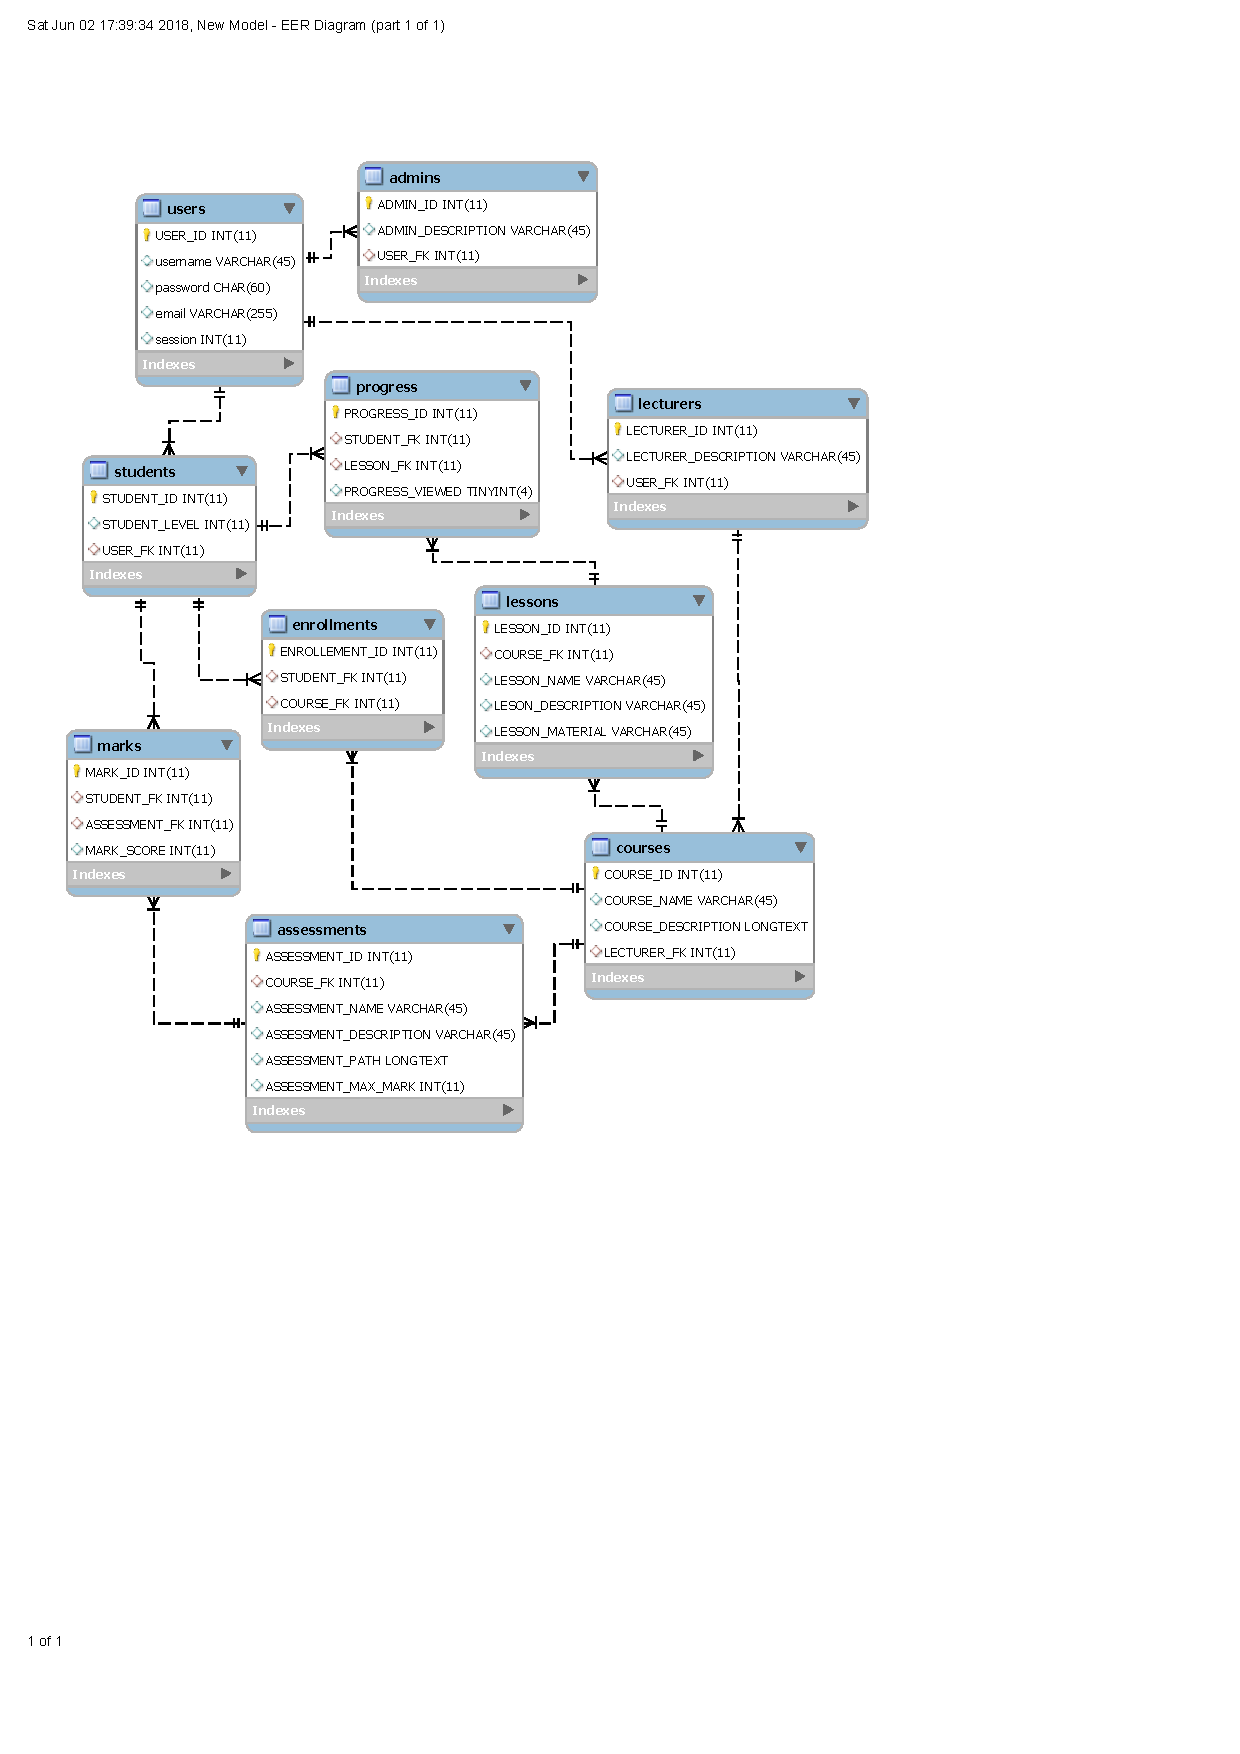
\includegraphics[scale = 0.95,trim = {0 10cm 6cm 2.5cm},clip]{./images/model.pdf} %lbrt
\caption{Database ERD}
\label{model}
\end{figure}

\section{Front-end}
The following section provide images of the website's user interface to illustrate the front-end of the completed site.
\subsection{Login and Register Interface}
The first page any user encounters is the login page (figure \ref{login}). If the current user does not have and account, the \textit{Signup}-link can be used to browse to the registration page (figure \ref{register}).

\newcommand{\picScale}{0.55}
\newcommand{\minipageWidth}{0.46\textwidth}

\begin{figure}[H]
\minipage[t]{\minipageWidth}
	\centering
	\fbox{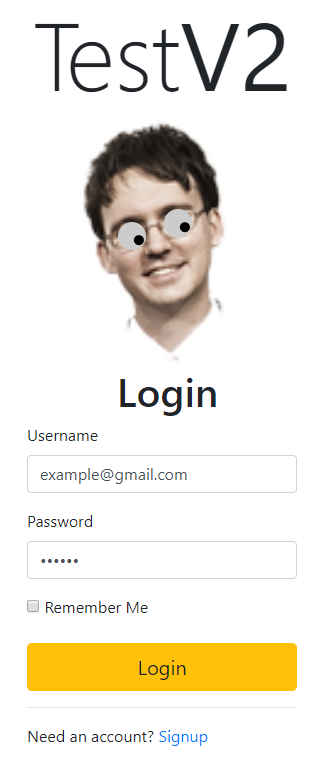
\includegraphics[scale = 0.6]{./images/login.png}}
	\caption{Login page}
	\label{login}
\endminipage\hfill
\minipage[t]{\minipageWidth}
	\centering
	\fbox{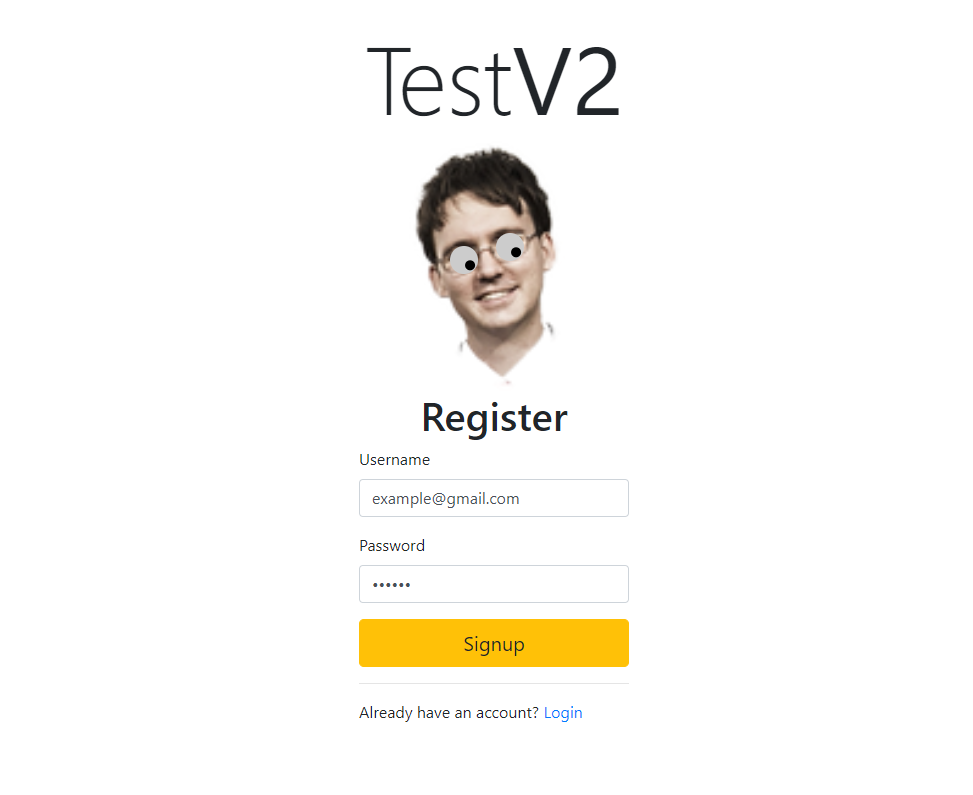
\includegraphics[scale = 0.6]{./images/register.png}}
	\caption{Register page}
	\label{register}
\endminipage
\end{figure}



\subsection{Lecturer Interface}
Upon signing in, lecturers are routed to the profile page where they can choose to create or add courses (figures \ref{createCourse} and \ref{addCourse}). If the lecturer clicks on one of the added courses, he is taken to a corresponding section for managing the particular course.

\begin{figure}[H]
\centering
\fbox{
\includegraphics[scale = 0.6]{./images/lecturerProfile.png}}
\caption{Lecturer profile page}
\label{lecturerProfile}
\end{figure}


\begin{figure}[H]
\minipage[t]{\minipageWidth}
	\centering
	\fbox{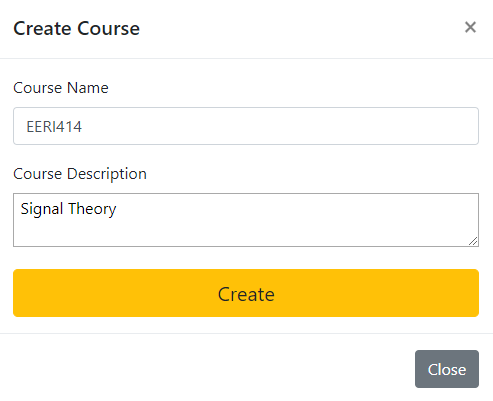
\includegraphics[scale = \picScale]{./images/createCourse.png}}
	\vspace{-0.2cm}
	\caption{Page for creating a course}
	\label{createCourse}
\endminipage\hfill
\minipage[t]{\minipageWidth}
	\centering
	\fbox{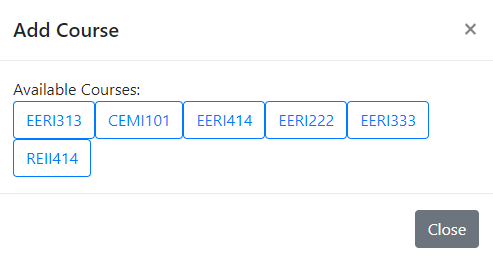
\includegraphics[scale = \picScale]{./images/addCourse.png}}
	\vspace{-0.2cm}
	\caption{Page for adding a course}
	\label{addCourse}
\endminipage
\end{figure}

Figure \ref{lecturerLessons} shows the page for creating and deleting lessons. The page shown in figure \ref{lecturerAssessments} is used to create new assessments (figure \ref{lecturerCreateAssessment}) and update student marks (figure \ref{lecturerUpdateMarks}). The page in figure \ref{lecturerGradebook} is used to view each student's marks for every assessment.

\begin{figure}[H]
\centering
\fbox{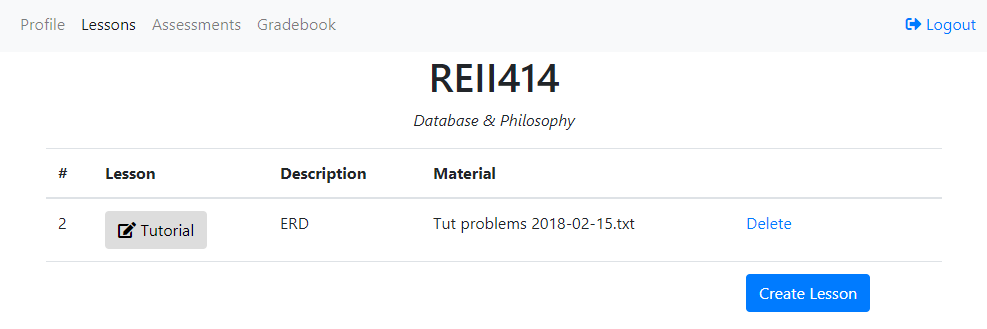
\includegraphics[scale = 0.6]{./images/lecturerLessons.png}}
\caption{Lecturer lessons page}
\label{lecturerLessons}
\end{figure}

\begin{figure}[H]
\centering
\fbox{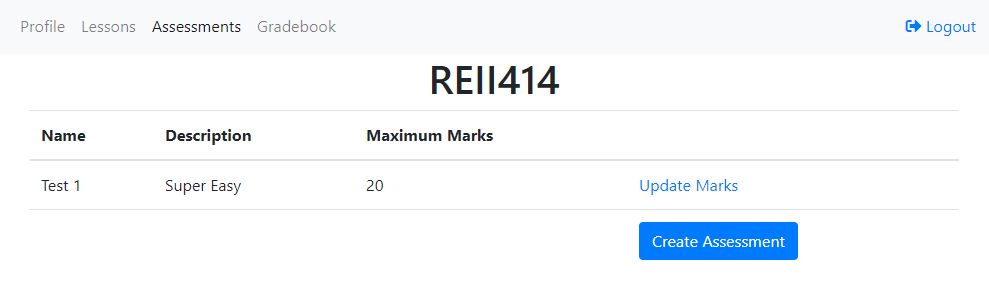
\includegraphics[scale = 0.6]{./images/lecturerAssessments.png}}
\caption{Lecturer assessments page}
\label{lecturerAssessments}
\end{figure}

\begin{figure}[H]
\centering
\fbox{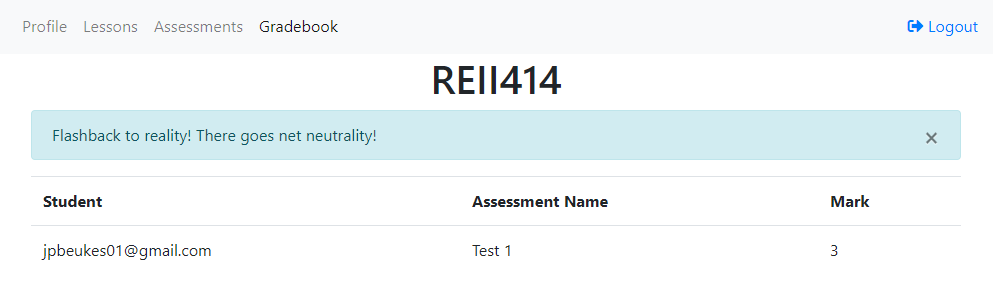
\includegraphics[scale = 0.6]{./images/lecturerGradebook.png}}
\caption{Lecturer gradebook page}
\label{lecturerGradebook}
\end{figure}

\begin{figure}[H]
\minipage[t]{\minipageWidth}
	\centering
	\fbox{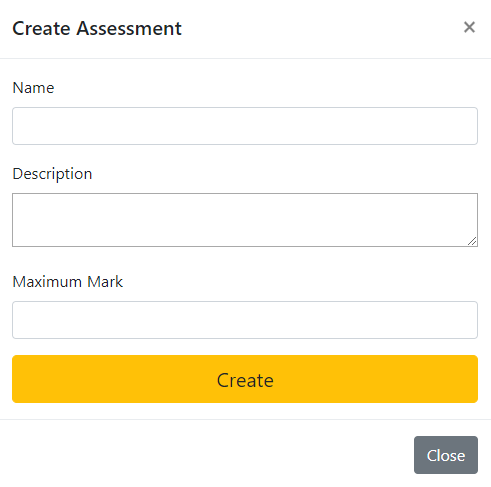
\includegraphics[scale = \picScale]{./images/lecturerCreateAssessment.png}}
	\vspace{-0.2cm}
	\caption{Creating assessments page}
	\label{lecturerCreateAssessment}
\endminipage\hfill
\minipage[t]{\minipageWidth}
	\centering
	\fbox{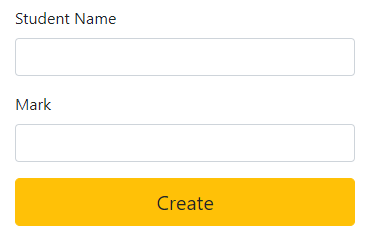
\includegraphics[scale = \picScale]{./images/lecturerUpdateMarks.png}}
	\vspace{-0.2cm}
	\caption{Update student marks page}
	\label{lecturerUpdateMarks}
\endminipage
\end{figure}



\subsection{Student Interface}
Students have the same interface as lecturers, except for the editing functionality. No add, update of delete privileges are given to students, aside from the option of adding courses to their site. The profile page for students are given in figure \ref{studentProfile}, but all other examples of student pages are omitted in favour of brevity.

\begin{figure}[H]
\centering
\fbox{
\includegraphics[scale = 0.6]{./images/studentProfile.png}}
\caption{Student profile page}
\label{studentProfile}
\end{figure}

\pagebreak
\section{Back-end}
\subsection{Sign up and Login}
The 'passport' package in Nodejs allows the site to handle sessions as well as cookies in an organised way. The session stores the current user's personal info inside his/her browser to allow for a personalised site.\\
The 'bcrypt' package allows the passwords to be encrypted in the database with the sha256 algorithm. This ensures that the system administrators can enter into the user's sites.\\
Figures \ref{cLocalSignup} and \ref{cLocallogin} can be summarised as, insert new user into database with encrypted password. The user logging in gets flashed error messages; should the details entered be wrong.
<<<<<<< HEAD
<<<<<<< HEAD
=======


\begin{figure}[H]
\centering
\fbox{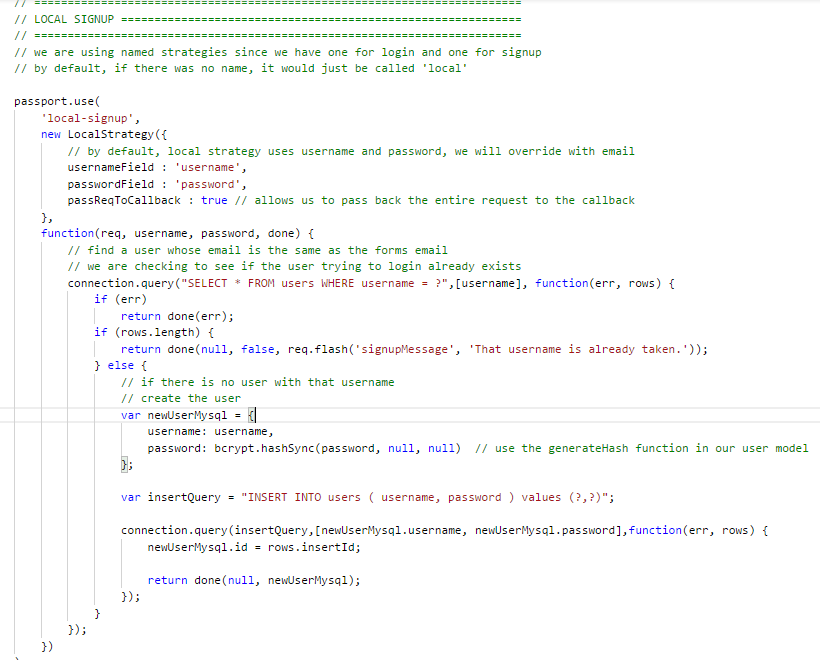
\includegraphics[width = 0.9\textwidth]{./images/cLocalSignup}}
\caption{Code: Local Sign-up}
\label{cLocalSignup}
\end{figure}

\begin{figure}[H]
\centering
\fbox{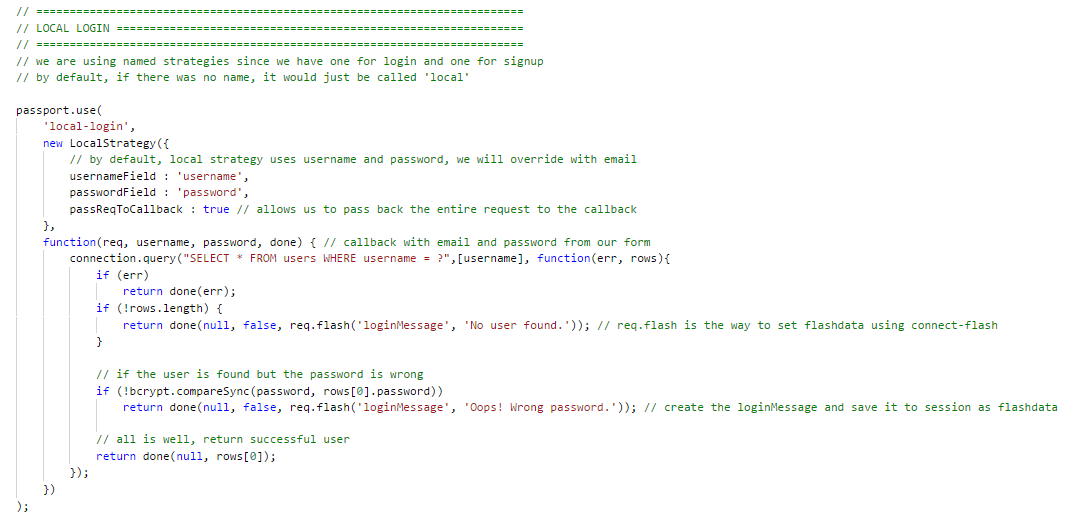
\includegraphics[width = 0.95\textwidth]{./images/cLocalLogin}}
\caption{Code: Local Login}
\label{cLocallogin}
\end{figure}

\subsection{Courses}
Courses can be created and edited by lecturers, whereas students can only view the courses. Figure \ref{cPostcourse} shows how a new course is added to the database. Figure \ref{ccourses} shows how the course and all of its content is retrieved as a JSON object from the database and rendered to the user.

\begin{figure}[H]
\centering
\fbox{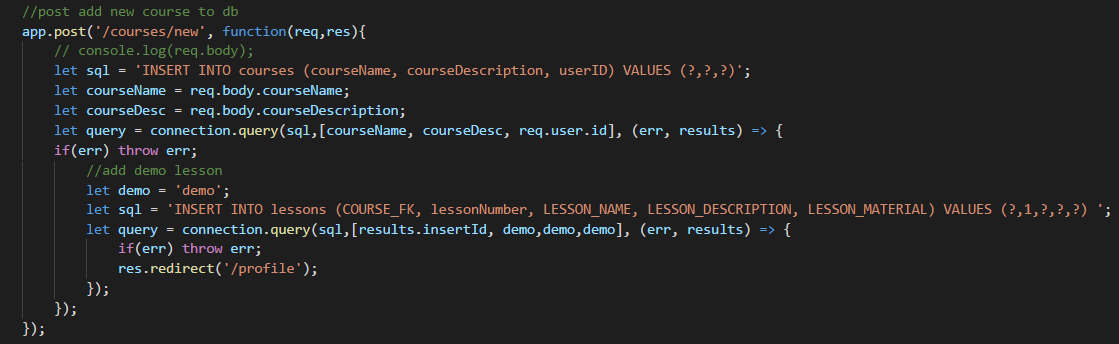
\includegraphics[width = 0.95\textwidth]{./images/cPostCourse}}
\caption{Code: Create new course}
\label{cPostcourse}
\end{figure}

\begin{figure}[H]
\centering
\fbox{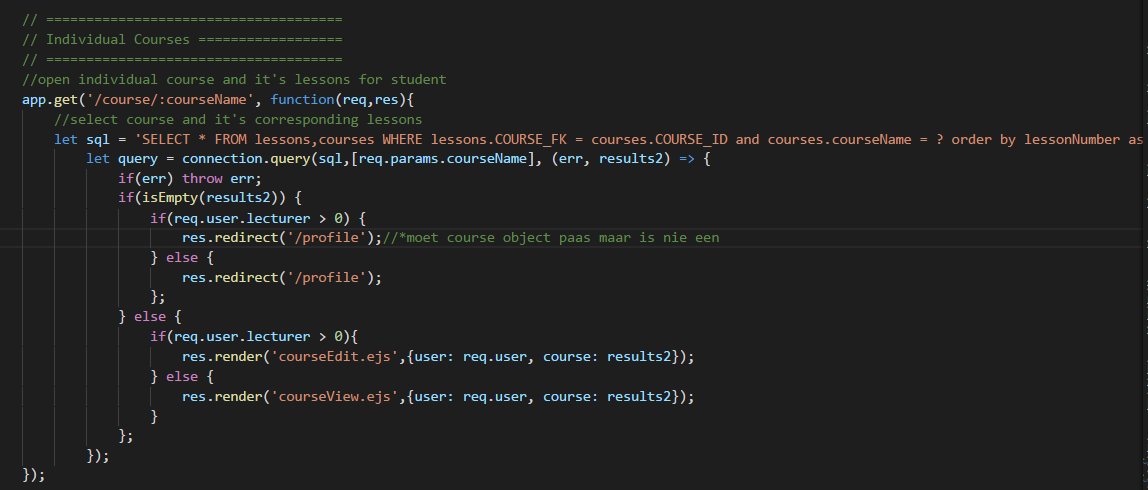
\includegraphics[width = 0.95\textwidth]{./images/cCourses}}
\caption{Code: Get Courses}
\label{ccourses}
\end{figure}

\subsection{Lessons}
The code in Figure \ref{cLessons} shows the post request when the lecturer creates a new lesson. The details of of the lesson is added with the files and are sent to the server and database for later retrieval.

\begin{figure}[H]
\centering
\fbox{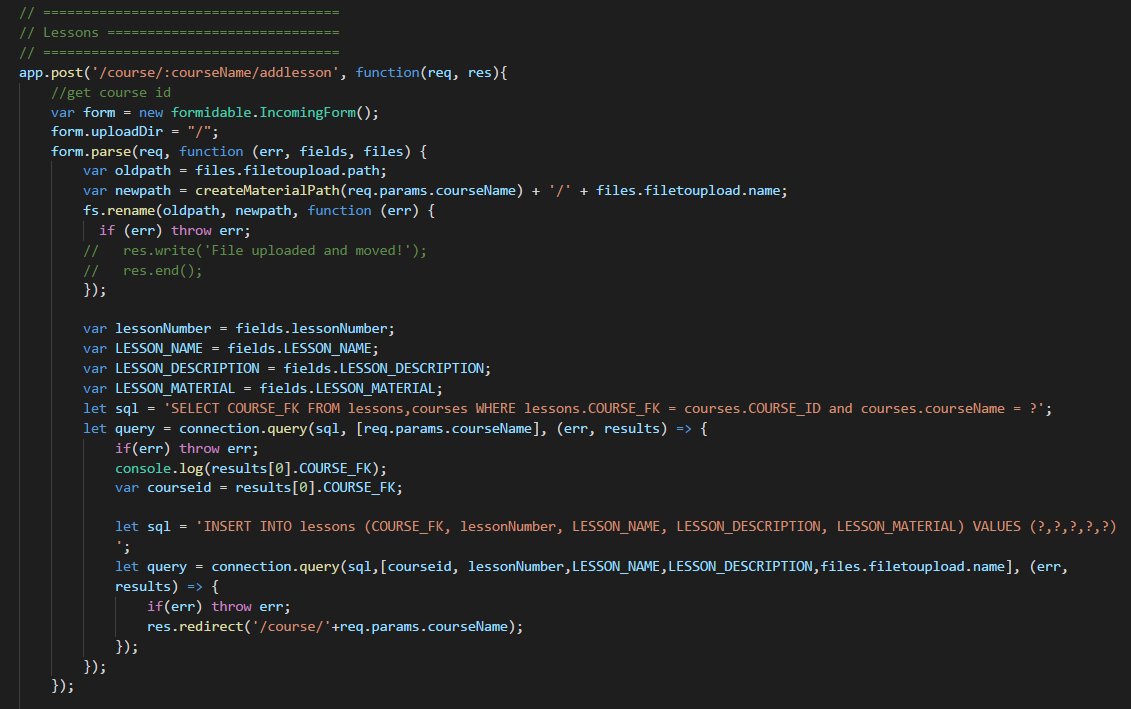
\includegraphics[width = \textwidth]{./images/clessons}}
\caption{Code: Create Lessons}
\label{cLessons}
\end{figure}


\subsection{Assessments}
The lecturer can add assessments to a course and enter the marks of the students for a specific assessment. Figure \ref{cAses} below shows how a new assessment is posted to the database and how marks are inserted for a specific user.

\begin{figure}[H]
\centering
\fbox{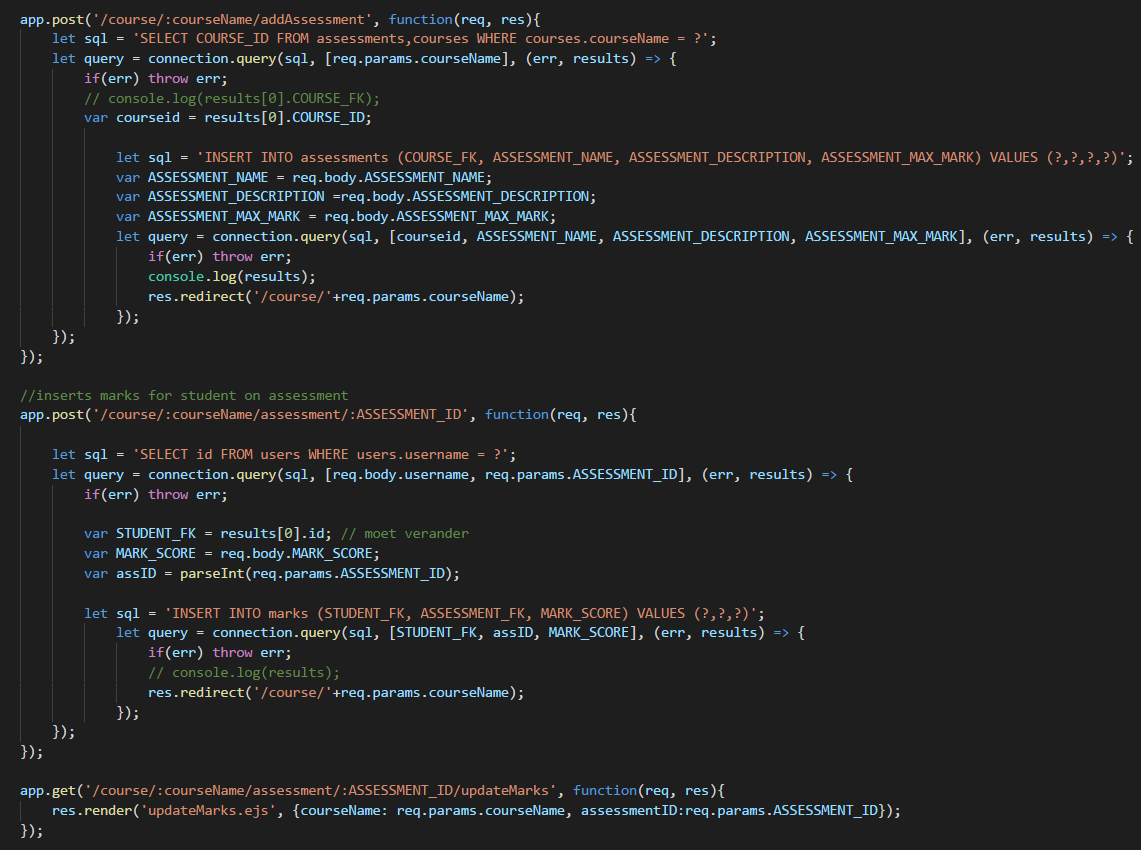
\includegraphics[width = \textwidth]{./images/cAssess}}
\caption{Code: Create and Update Marks for Assessments}
\label{cAses}
\end{figure}


=======
>>>>>>> 964572605eb935cefc43296bedd5af14ec12e368


\begin{figure}[H]
\centering
\fbox{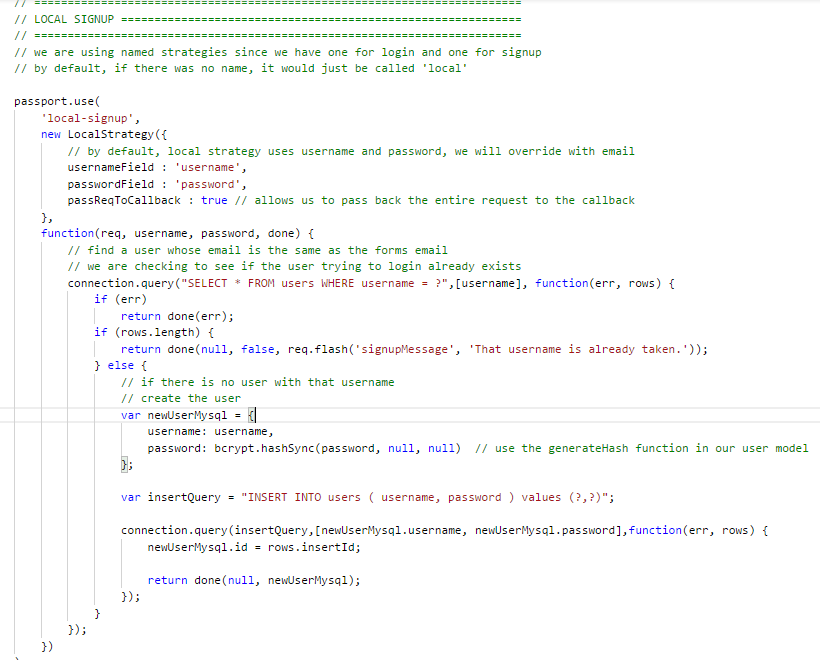
\includegraphics[width = 0.9\textwidth]{./images/cLocalSignup}}
\caption{Code: Local Sign-up}
\label{cLocalSignup}
\end{figure}

\begin{figure}[H]
\centering
\fbox{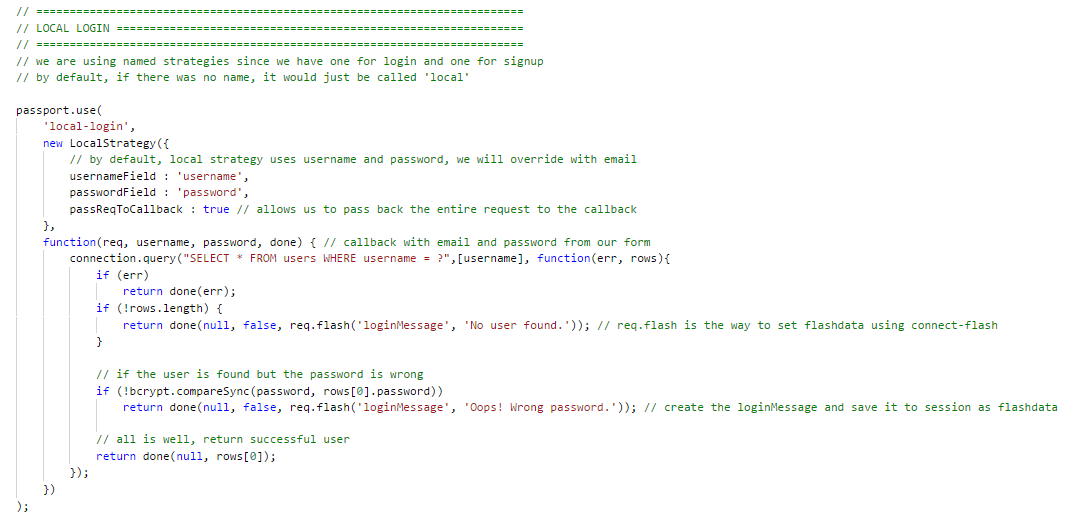
\includegraphics[width = 0.95\textwidth]{./images/cLocalLogin}}
\caption{Code: Local Login}
\label{cLocallogin}
\end{figure}

\subsection{Courses}
Courses can be created and edited by lecturers, whereas students can only view the courses. Figure \ref{cPostcourse} shows how a new course is added to the database. Figure \ref{ccourses} shows how the course and all of its content is retrieved as a JSON object from the database and rendered to the user.

\begin{figure}[H]
\centering
\fbox{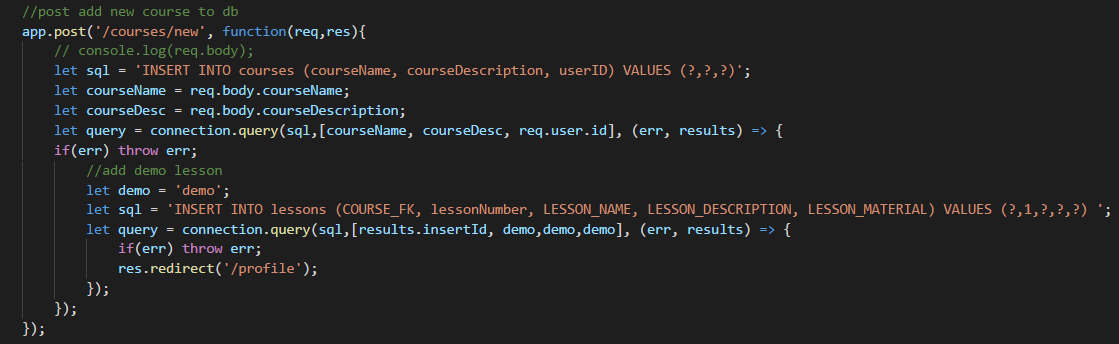
\includegraphics[width = 0.95\textwidth]{./images/cPostCourse}}
\caption{Code: Create new course}
\label{cPostcourse}
\end{figure}

\begin{figure}[H]
\centering
\fbox{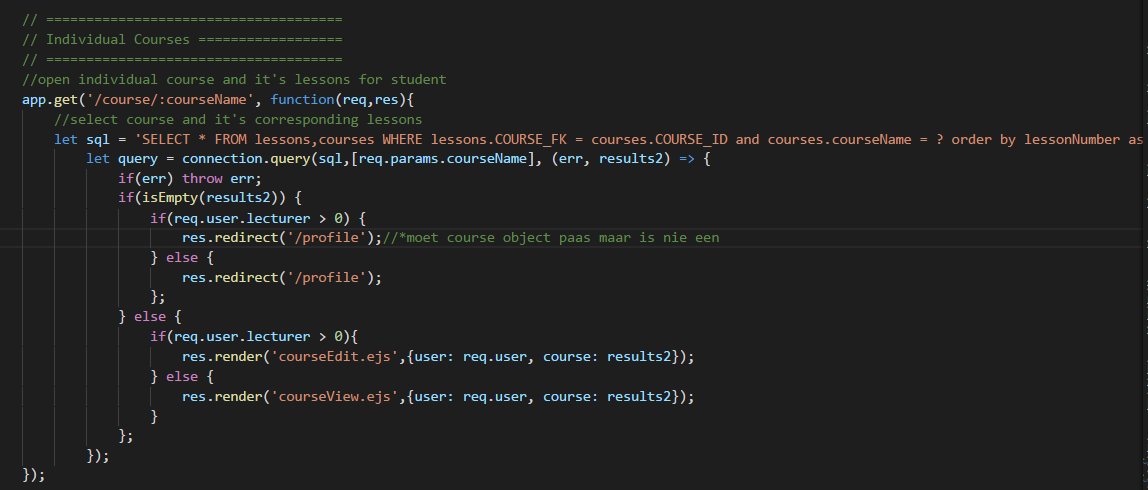
\includegraphics[width = 0.95\textwidth]{./images/cCourses}}
\caption{Code: Get Courses}
\label{ccourses}
\end{figure}

\subsection{Lessons}
The code in Figure \ref{cLessons} shows the post request when the lecturer creates a new lesson. The details of of the lesson is added with the files and are sent to the server and database for later retrieval.

\begin{figure}[H]
\centering
\fbox{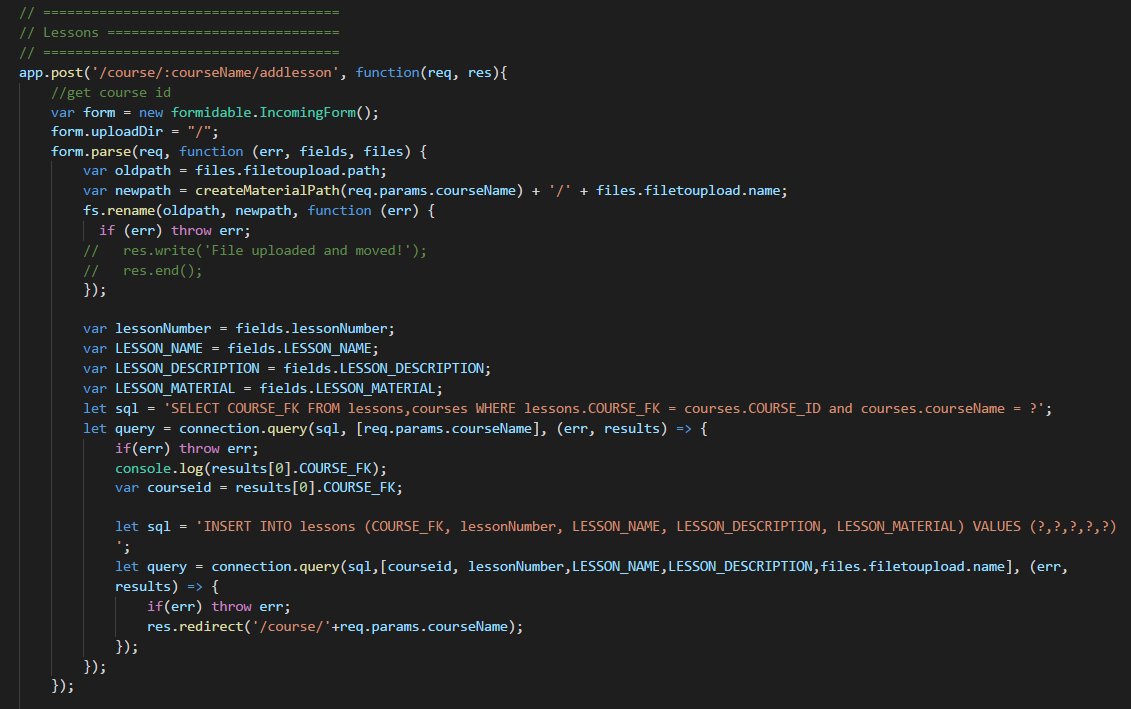
\includegraphics[width = \textwidth]{./images/clessons}}
\caption{Code: Create Lessons}
\label{cLessons}
\end{figure}


\subsection{Assessments}
The lecturer can add assessments to a course and enter the marks of the students for a specific assessment. Figure \ref{cAses} below shows how a new assessment is posted to the database and how marks are inserted for a specific user.

\begin{figure}[H]
\centering
\fbox{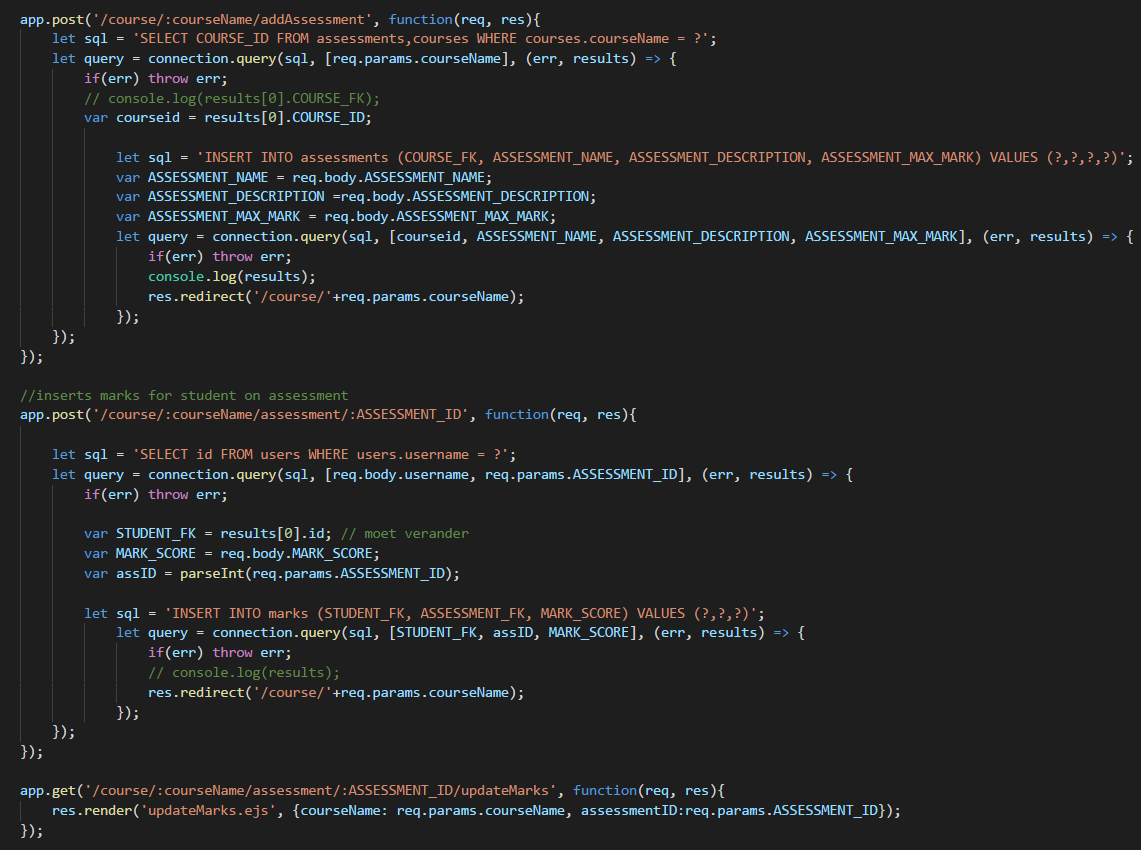
\includegraphics[width = \textwidth]{./images/cAssess}}
\caption{Code: Create and Update Marks for Assessments}
\label{cAses}
\end{figure}


>>>>>>> a996558f8669738c04ad45915fcc0079d4103839

\begin{figure}[H]
\centering
\fbox{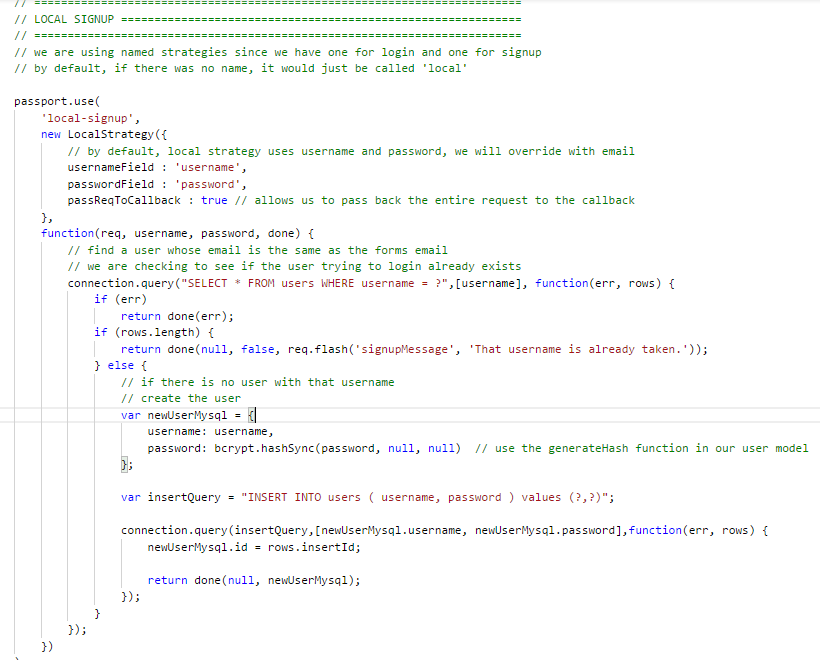
\includegraphics[width = 0.9\textwidth]{./images/cLocalSignup}}
\caption{Code: Local Sign-up}
\label{cLocalSignup}
\end{figure}

\begin{figure}[H]
\centering
\fbox{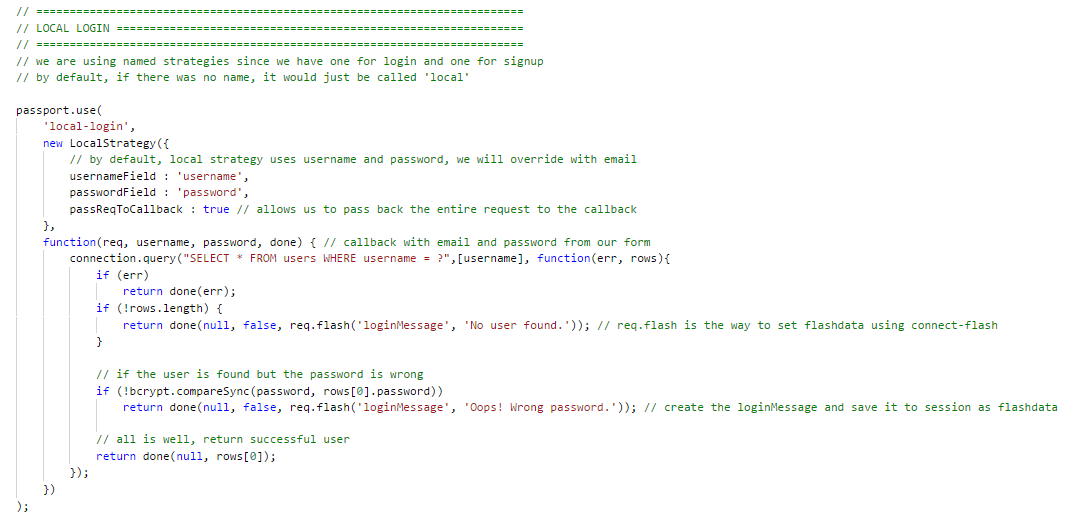
\includegraphics[width = 0.95\textwidth]{./images/cLocalLogin}}
\caption{Code: Local Login}
\label{cLocallogin}
\end{figure}

\subsection{Courses}
Courses can be created and edited by lecturers, whereas students can only view the courses. Figure \ref{cPostcourse} shows how a new course is added to the database. Figure \ref{ccourses} shows how the course and all of its content is retrieved as a JSON object from the database and rendered to the user.

\begin{figure}[H]
\centering
\fbox{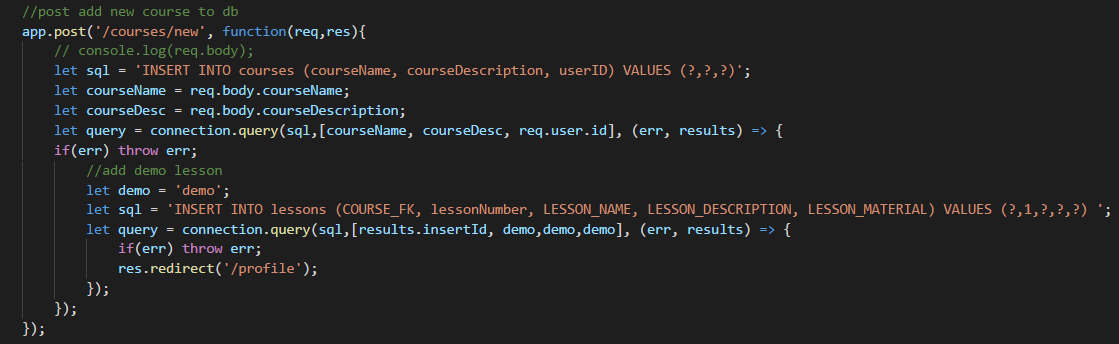
\includegraphics[width = 0.95\textwidth]{./images/cPostCourse}}
\caption{Code: Create new course}
\label{cPostcourse}
\end{figure}

\begin{figure}[H]
\centering
\fbox{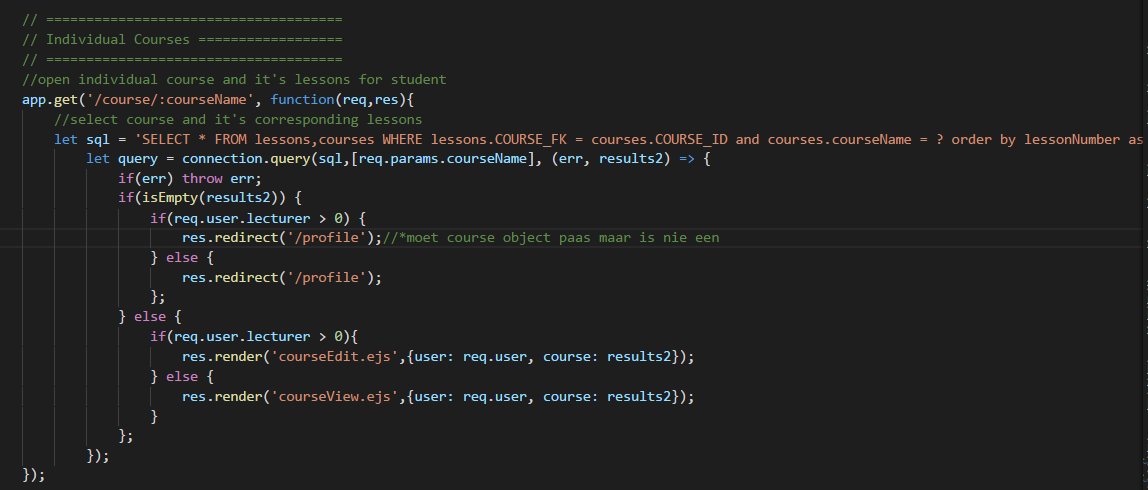
\includegraphics[width = 0.95\textwidth]{./images/cCourses}}
\caption{Code: Get Courses}
\label{ccourses}
\end{figure}

\subsection{Lessons}
The code in Figure \ref{cLessons} shows the post request when the lecturer creates a new lesson. The details of of the lesson is added with the files and are sent to the server and database for later retrieval.

\begin{figure}[H]
\centering
\fbox{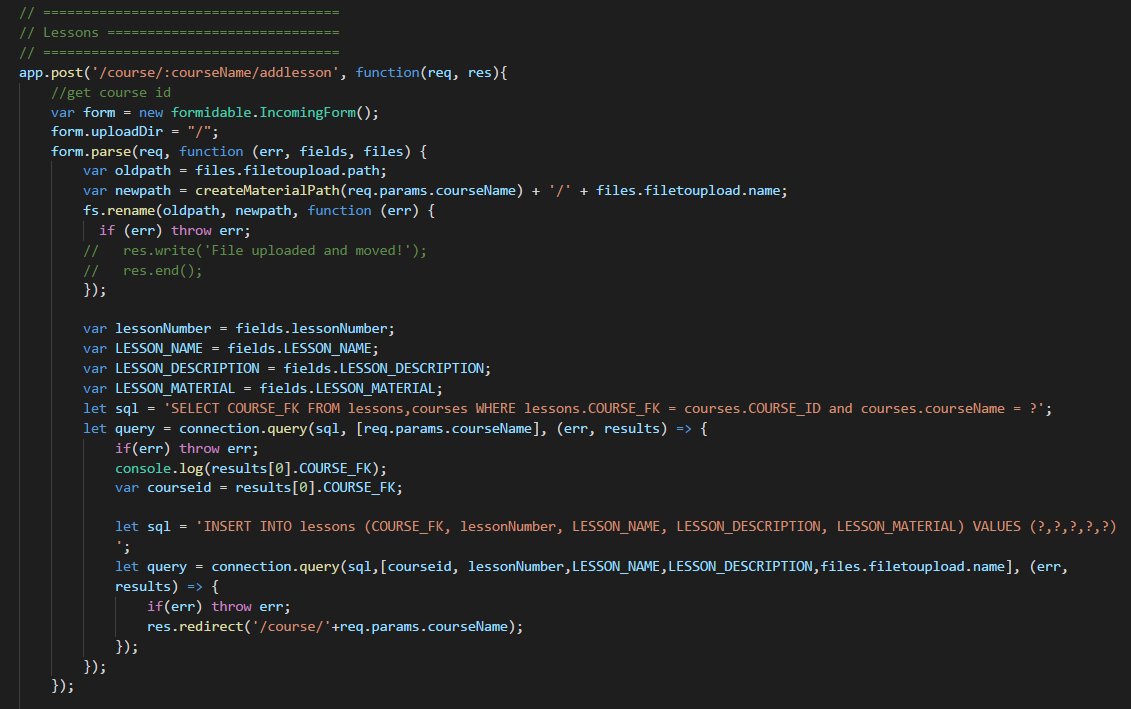
\includegraphics[width = \textwidth]{./images/clessons}}
\caption{Code: Create Lessons}
\label{cLessons}
\end{figure}


\subsection{Assessments}
The lecturer can add assessments to a course and enter the marks of the students for a specific assessment. Figure \ref{cAses} below shows how a new assessment is posted to the database and how marks are inserted for a specific user.

\begin{figure}[H]
\centering
\fbox{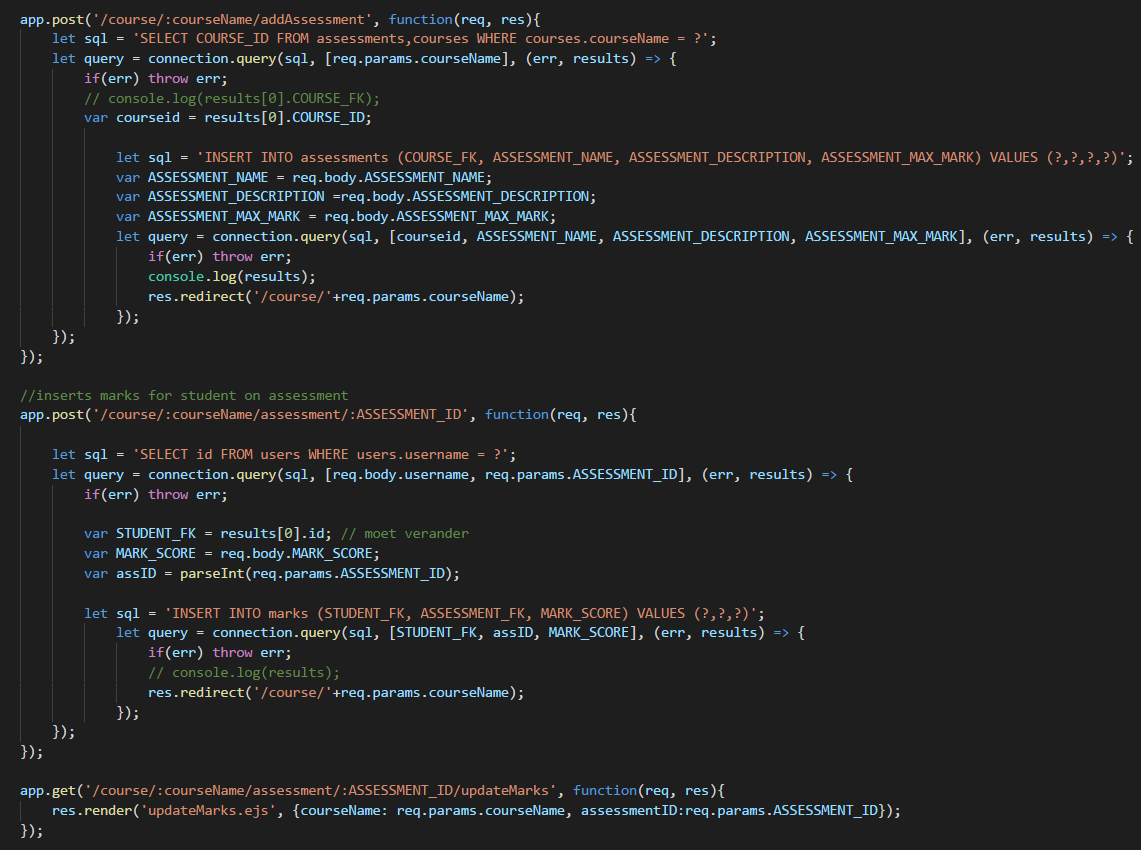
\includegraphics[width = \textwidth]{./images/cAssess}}
\caption{Code: Create and Update Marks for Assessments}
\label{cAses}
\end{figure}


\subsection{Grade-book}
Lastly the grade-book is split into two types, one for students and one for lecturers. The student grade book only gets the student's mark for all the assessments in that course. The lecturer's grade book show all the students and their respective mark for all of the assessments. 

\begin{figure}[H]
\centering
\fbox{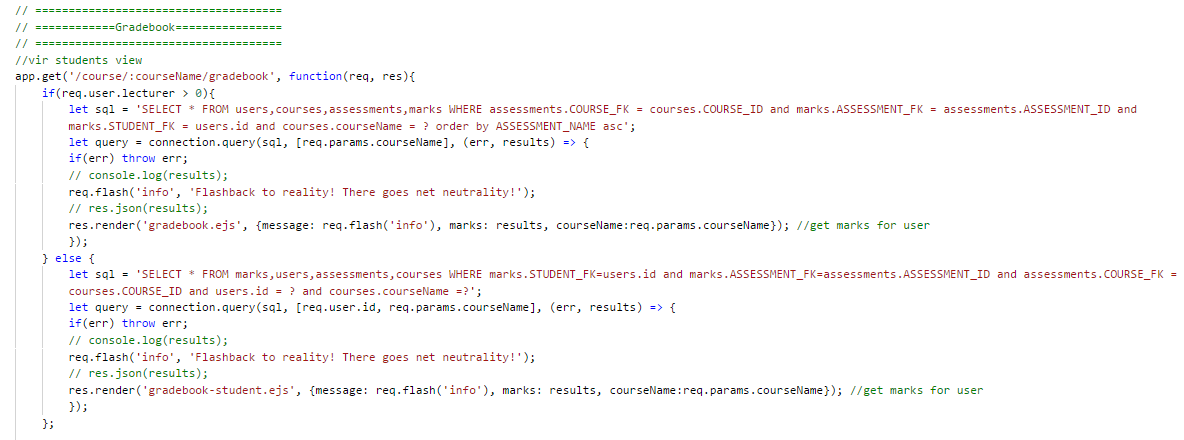
\includegraphics[width = \textwidth]{./images/cGrade}}
\caption{Code: Grade book}
\label{cGrade}
\end{figure}


%\begin{figure}[H]
%\centering
%\includegraphics[scale = 0.35]{./images/motorSchem.png}
%\caption{(a) Electrical diagram of a DC motor. (b) Sketch of DC motor \cite{dorf}.}
%\label{motorSchem}
%\end{figure}


%\newcommand{\picScale}{0.4}
%\newcommand{\minipageWidth}{0.46\textwidth}
%
%\begin{figure}[H]
%\minipage[t]{\minipageWidth}
%	\centering
%	\fbox{\includegraphics[scale = \picScale]{./images/stepResponse.png}}
%	\vspace{-0.2cm}
%	\caption{Graph showing the DC motor's step response.}
%	\label{stepResponse}
%\endminipage\hfill
%\minipage[t]{\minipageWidth}
%	\centering
%	\fbox{\includegraphics[scale = \picScale]{./images/naturalResponse.png}}
%	\vspace{-0.2cm}
%	\caption{Graph showing the DC motor's natural response.}
%	\label{naturalResponse}
%\endminipage
%\end{figure}

\pagebreak
\section{Conclusion}

\subsection{Strengths}
By using the Node js for developing instead of PHP creates a much more developer friendly environment. Using the Node js mysql library allows the developer to create queries that is already safe from SQL injections. Passwords are encrypted with sha256 inside the database. The structure of the database is easily expandable. All of the user's data is stored in a session and cookies, alleviating unnecessary requests to the server and making the website more personalised.   

\subsection{Flaws}
An automatic assessment creator and marker would be better than manually typing in the marks students received for their tests. Manually typing in each student's mark for each assessment could become slow and tedious. 

\subsection{Improvements}
Future versions of the website could include a section for online assessments, where lecturers are able to create new tests and students can complete existing tests. The website must then be able to evaluate the student's answers and update their marks.

The current version of the website can only be accessed via a local network. To launch the site for global use, a domain name have to be acquired.\\

A better developing scheme would be to use a MVC (Model View Controller) structure. 

\subsection{Techniques Learned}
HTTP post and get requests where used extensively in this project. Hence, much knowledge of the protocol and its header structure where acquired. \\

How to set up a database and preform queries that have relationship with each other.\\

How to create a website with HTML, Javascript and CSS, whilst providing a user friendly experience to the users.


\addcontentsline{toc}{section}{References}
\nocite{*} % include this when you want to have all your (Jabref) references shown. comment out if you want only the ones that are used in the document diplayed.
\bibliographystyle{IEEEtran}
\bibliography{./ref} % the path to your filename of your .bib library


\end{document}
